\documentclass[12pt, titlepage]{article}
\title{PWS AI}
\author{Maarten Stremler \and Ivar de Bruin \and Jaap de Jong}
\PassOptionsToPackage{hyphens}{url}
\usepackage{amssymb, amsmath}
\usepackage{hyperref}
\usepackage{listings}
\usepackage{color}
\usepackage{tikz}

%forces a pagebreak before a new section
\let\oldsection\section
\renewcommand\section{\clearpage\oldsection}

%defines the look of the code we use
\definecolor{dkgreen}{rgb}{0,0.6,0}
\definecolor{gray}{rgb}{0.5,0.5,0.5}
\definecolor{mauve}{rgb}{0.58,0,0.82}

\lstset{frame=tb,
    language=Java,
    aboveskip=3mm,
    belowskip=3mm,
    showstringspaces=false,
    columns=flexible,
    basicstyle={\small\ttfamily},
    numbers=none,
    numberstyle=\tiny\color{gray},
    keywordstyle=\color{blue},
    commentstyle=\color{dkgreen},
    stringstyle=\color{mauve},
    breaklines=true,
    breakatwhitespace=true,
    tabsize=3
}

\setlength{\parindent}{0pt}
%Door deze regel springt de eerste regel van
%elke alinea niet meer steeds een stukje in.
\setlength{\parskip}{\baselineskip}
%Door deze regel wordt tussen de alinea's steeds
%een regel overgeslagen.

\tikzset{%
    every neuron/.style={
        circle,
        draw,
        minimum size=1cm
    },
    neuron missing/.style={
        draw=none, 
        scale=4,
        text height=0.333cm,
        execute at begin node=\color{black}$\vdots$
    },
}


\begin{document}
    \maketitle
    \tableofcontents
    
\section{Introduction}
    In recent years, we have seen enormous advances in the field of AI. In 2016 Google's DeepMind AI beat the reigning world champion at Go, one of the most difficult games there is\cite{byford16}. Go has a possibility space which is exponentially larger than that of, for instance, chess. In the same year it was announced that Microsoft had built an AI which surpassed humans when it came to speech recognition.
    Most, if not all, of these huge steps forward have been made possible due to an exponential rise in computing power and the usage of GPUs for massive parallel computing in the last few years.
    \\
    \\
    Another very important factor is the revival of the neural net. This particular form of AI was devised in the late forties. In the seventies they fell out of grace, but with the advance of computing power, so called ‘deep’ neural networks became feasible and ever since 2010, neural networks have dominated the field of AI.\cite{kuzovkin16}\cite{foote17} Artificial Intelligence usually makes headlines when it has beaten us humans in something. Often it is a board game or some other type of game. Because of this constant comparison between humans and AI, we wanted to compare them on another level. An essential function of our brain is recognizing peoples faces. This is, among other things, very important in our social life. Because of that, our research will focus on facial recognition by AI.
    
    \subsection{Main Question}
    The main goal of this research is to answer the following question:
    \begin{center}
        \textit{What is the difference in speed and effectivity between humans and artificial intelligence, when it comes to facial recognition?}
    \end{center}
    
    \subsection{Demarcation}
    For this research, an AI capable of recognizing faces will be built and tested against human intelligence. This will be done by giving the AI and one of the researchers a fixed amount of time to classify as many pictures of human faces as possible. After the time is over, speed (how many pictures were processed) and effectiveness (what part of the processed pictures has been classified correctly) will be measured, in order to evaluate the performance of both the AI and its human counterpart.
    \subsubsection{Specificity}
    The concepts discussed in the main question are very described in a specific manner. We should however remark that the term 'Artificial Intelligence' is not very specific, because the exact structure of the AI is not yet known at this moment. We will give more details about this in phase 4.
    \subsubsection{Measurability}
    The performance of the AI and the human test subjects will be measured by giving them a certain amount of tests. We will log the amount of right and wrong answers and, if relevant, the amount of time the subject needs to finish the test. After that, the AI could possibly be trained for other tasks, such as playing chess. Just like facial recognition there are a lot of different methods to compare performance between human and AI here as well.
    \subsubsection{Acceptability}
    There is enough time to design and build the AI. Researches can program at home and at school. The training of the AI can be paused without corrupting any data, so the AI can be trained with big data sets without having to let a computer run ceaselessly for a certain amount of days. Running an AI is not dangerous for the computer or the network.
    \subsubsection{Realistic}
    Researchers possess enough mathematical and programming knowledge to build the AI. There is still some uncertainty about the time needed to build a working AI.
    \subsubsection{Time-bound}
    The duration of a test is not of interest, as long as human and AI get the same amount of time to finish the test. We presume this won't take a lot of time. We aim to build a relatively fast AI that should outperform humans at least if we look at the time required to recognize someone. The designing, building and testing of the AI, however, is very likely to require a lot more time.  
   
    \section{Sub-questions}
    
    
    \subsection{There are lots of different ways of building neural networks and there are lots of hyper-parameters to configure. Which type of neural network works best for our purposes?}
    
    \bigskip
    \subsection{What can we say about the differences between humans and AI when it comes to mastering certain tasks?}
    \subsubsection{What is the difference in time required to master a certain task?}
    \subsubsection{What is the difference when it comes to the amount of examples required to master a certain task?}
    
    \bigskip
    \subsection{What is the difference in performance between humans and AI?}
    \subsubsection{What is the difference when it comes to the amount of successfully recognized images?}
    \subsubsection{Are humans or AI better at recognizing linking pictures of people at different ages, or which ‘system’ is more sensitive when it comes to the aging process?}
    
    \bigskip
    \subsection{Can an AI capable of facial recognition also be trained to perform other tasks?}
    \subsubsection{Can it crack Captchas?}
    \subsubsection{Can it be taught to play a simple (board) game?}
    \subsubsection{Can we let the AI differentiate between different kinds of input, so that one and the same AI is capable of performing multiple tasks?}
    
    
    \subsection{Even if the AI has a lower success rate recognizing faces on pictures, it will probably still be way faster than the average human. In which situations would this advantage of being fast be of such importance, that the disadvantage when it comes to accuracy can be neglected?}
    
    \section{Research method}
    \subsection{Literature research as preparation for building the AI}
    Lots of reliable sources were found stating that convolutional neural nets are the state of the art when it comes to image recognition\cite{gu}\cite{imageRecognition17}. In fact, we were unable to find any recent research on computer vision which didn’t include something about neural nets. This is why neural nets will be the AI technique used and why the focus of our literature research is going to lie on the specifics of the neural net we are going to build.
    
    \bigskip
    Information about neural nets will come mainly from Wikipedia and YouTube, though there are also a few blogs containing very valuable information on the back propagation algorithm. Books and research articles on neural nets usually don’t provide any information needed for actually building and training neural nets, but rather information on the best activation functions, new complicated ways to better train neural nets and so on.  This is all very interesting when you are trying to improve an existing neural net or when you have a lot of experience building neural nets, but when making a first-time build, all this extra information isn't really needed.
    \bigskip
    Though the reliability of used sources is obviously very important, there is fail-safe in place which isn’t present in most research projects. When two contradicting methods of implementing neural nets are found, both can be implemented and tested. This is why Wikipedia and YouTube are regarded as reliable enough for the purposes of our research.
    
    \subsection{Comparing the AI to humans}
    After an AI has been built which is able to compare pairs of pictures and tell us whether they are of the same person or not, a series of tests and experiments will be conducted in order to compare the AI to humans and to test the limitations of the AI. The research will be experimental.
    
    \bigskip
    When comparing humans to AI, we should not forget that the strengths of AI are different to those of humans. Therefore, it is best to conduct a wide range of tests, looking at different aspects of facial recognition.
    
    \bigskip
    Only the first two tests are real tests of the AI, comparing it to humans. Test 3 and test 4 simply state that the first two tests will be conducted on different people, different AIs and with multiple different samples in such way that other properties of the AI can be researched. The four tests are quantitative in nature, while the two experiments lean toward the qualitative side.
    
    \bigskip
    We conclude with two proposing two experiments which can be conducted on a working facial recognition AI. All our research will be done using the observational method. There are also some existing datasets (pictures of faces) that will be used as raw input to the AI for training purposes.
    
    \subsubsection{Percentage of given pictures recognized}
    It is expected that, in general, humans are better at picture recognition than AI when it comes to the percentage of pictures recognized. Test samples will be generated by picking a list of pictures and forming all possible unordered pairs of pictures. Then, both human and AI are given as much time as they need to classify all pairs as ‘same person’ or ‘different person’, though in reality, the AI won't take more than a second, while a human may take up to a few minutes. After the entire sample has been classified, data like the amount of false negatives and the amount of false positives will be computed and visualized in graphs and tables.
    
    \subsubsection{Amount of pictures recognized in a given period of time}
    While humans are more accurate when it comes to facial recognition, the AI will be much and much faster, something to take into account when comparing AI to humans. First, a sample of unordered pairs of pictures will be generated. Then both humans and AI will be given a fixed amount of time, say two minutes, to classify as many pictures as possible. We must ensure that the sample is so large, that the AI won't be able to classify all the pictures in the sample within the given time. Afterwards, different statistical quantities like the percentage of false negatives and the percentage of false positives will be computed and put into tables and graphs for visualization purposes.
    
    \subsubsection{The difference in learning time}
    For humans, the ability to recognize faces is nearly fully developed around the age of one. AI, on the other hand, only takes a couple of hours of training to reach a state in which it performs reasonably well. All the following tests will be conducted on different age groups and on one and the same AI in different stages of its learning process.
    
    \bigskip
    Related to this test is the difference in how effective the learning data is being used. We can approximate the total amount of pictures a person has been exposed to in their life. We will compare this to the total amount of pictures the AI has used as training data.
    
    \subsubsection{Recognizing people in different stages in their lives}
    When people age, their face changes. We will test whether the AI is able to cope with this difference and if it is indeed able to classify two faces (of the same person, but at different ages) as being one and the same. For this purpose, we will conduct the above tests with multiple sample sets, some of which will contain pictures taken around the same time and some of which will contain pictures taken at many different times.
    
    \subsubsection{Teaching the AI other tasks than facial recognition}
    After all the previous tests have been conducted, an attempt will be made to teach the AI other tasks, such as playing a board game, like chess or checkers. This will be done as follows: when it is the AI’s turn to make a move, a computer program will perform all possible moves and compute all possible boards. Then, theses boards will be compared to each other with the AI, which will classify all pairs as ‘board one is better’ or ‘board two is better’. This way, the best possible next board will be computed and the move that leads to this board is performed. Now, we can let two instances of the AI play against each other, until they are proficient enough to face a human opponent.
    
    \subsubsection{One AI performing multiple tasks}
    If the previous experiment is completed successfully, an attempt will be made to create a single AI capable of performing multiple tasks. The AI will consist of multiple neural networks, one of which will take the raw input and decide the class of the problem (for example, if input is two pictures of chessboards, the AI will have output which one is the best one. If the input is two pictures of faces, the AI will have to return whether the pictures are of the same face or not). Then, the input data will be run through the appropriate neural net and the output will be returned. The performance of this AI will compared to the multiple AIs who each perform a single one of the tasks the more general AI can perform.
    
    \section{Convolutional neural networks explained}
    Before giving all the details of a convolutional neural net, it is best to take a look at the slightly less complicated classical artificial neural net. After these have been explained in some detail, the concept behind convolutional neural networks will seem more natural and certain design desicions will appear as obvious.
    
    \subsection{Classical neural networks}
    A classical artificial neural network takes in an input vector of a specific size and outputs an output vector of another specific size. The architecture of a neural net was originally based on the human brain with its neurons and connections between them. A network can be represented by some directed graph such as this one:    \\\\
    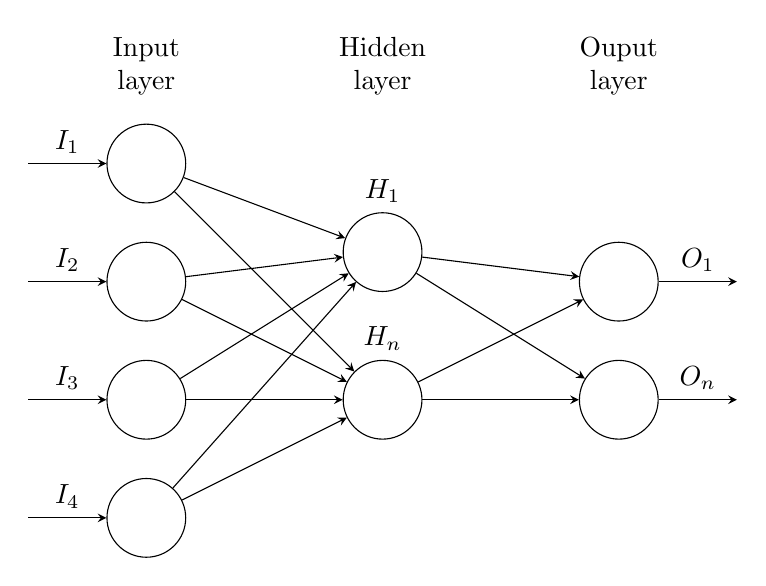
\begin{tikzpicture}[x=1.5cm, y=1.5cm, >=stealth]
    
    \foreach \m/\l [count=\y] in {1,2,3,4}
    \node [every neuron/.try, neuron \m/.try] (input-\m) at (0,2.5-\y) {};
    
    \foreach \m [count=\y] in {1,2}
    \node [every neuron/.try, neuron \m/.try ] (hidden-\m) at (2,2-\y*1.25) {};
    
    \foreach \m [count=\y] in {1,2}
    \node [every neuron/.try, neuron \m/.try ] (output-\m) at (4,1.5-\y) {};
    
    \foreach \l [count=\i] in {1,2,3,4}
    \draw [<-] (input-\i) -- ++(-1,0)
    node [above, midway] {$I_\l$};
    
    \foreach \l [count=\i] in {1,n}
    \node [above] at (hidden-\i.north) {$H_\l$};
    
    \foreach \l [count=\i] in {1,n}
    \draw [->] (output-\i) -- ++(1,0)
    node [above, midway] {$O_\l$};
    
    \foreach \i in {1,...,4}
    \foreach \j in {1,...,2}
    \draw [->] (input-\i) -- (hidden-\j);
    
    \foreach \i in {1,...,2}
    \foreach \j in {1,...,2}
    \draw [->] (hidden-\i) -- (output-\j);
    
    \foreach \l [count=\x from 0] in {Input, Hidden, Ouput}
    \node [align=center, above] at (\x*2,2) {\l \\ layer};
    
    \end{tikzpicture}
    \\
    This particular network takes an input vector of size $4$ and has output vectors of size $2$. This can be deduced from the fact that the \textit{input layer} of the network has $4$ nodes, while the \textit{output layer} contains $2$ nodes. Every node has its own floating-point value between $0$ and $1$, similar to the electric charge of the neurons in the human brain. In between the input- and output layers, there can be multiple so-called \textit{hidden layers}.
    
    When computing the output vector for a given input vector, the procedure is as follows: set the values of the nodes in the input layer equal to the values in the input vector. Then we compute the values of the other nodes layer by layer. For each node in a layer, we look at all the incoming connections from the previous layer (represented by the arrows in the graph). Each of these connections has some number associated with it representing the 'thickness' of the connection between the two 'neurons', called the \textit{weights}. We take the values of all the nodes in the previous layer connected to our node and multiply them with their respective weights and add up the results. Then the result is normalized between $0$ and $1$ by running it trough a special mathematical function, usually the sigmoid function, which is defined as:
    \begin{equation*}
    \sigma(z) = \frac1{1+e^{-z}}
    \end{equation*}
    The value which the sigmoid gives back is the value of our node.
    
    For example, let's say that in our example network we have$I_1=0,5$, $I_2=0,8$, $I_3=0,1$ and $I_4=0,1$  and for the weights $w_{I_1,H_1}=2$, $w_{I_2,H_1}=0,3$, $w_{I_3,H_1}=0.7$ and $w_{I_4,H_1}=5$. In order to compute the value of $H_1$, we first multiply the values of $I_1$, $I_2$, $I_3$ and $I_4$ by their respective weights and add them all up:
    \begin{equation*}
    0,5\cdot 2 + 0,8\cdot 0,3 + 0,1\cdot 0,7 + 0,1\cdot 5 = 1,81
    \end{equation*}
    Finally we run it through the sigmoid function, giving the value of $H_1$ as $\sigma(1,81)\approx 0,86$.
    
    The original inspiration behind neural networks was the human brain. Later, it was proven by George Cybenko \cite{cybenko} that neural networks with enough layers and correct weights could approximate almost any function, meaning that artificial neural networks could theoretically be trained to compute anything, given all the necessary input. It should be remarked that in practice this is impossible, since it requires an enormous amount of time and resources to find the right weights for large networks. 
    
    When discussing the process of finding the right weights for a network (this process is called \textit{training}), it will prove useful to have a mathematical model of a neural net. The usual model is as follows:
    \begin{itemize}
        \item Every layer of the network is assigned a number from $0$ to $L$, where the input layer has index $0$, the output layer has index $L$ and the hidden layers have indices $1,2,\ldots,L-2,L-1$.
        \item For any layer $l$, the amount of nodes in that particular layer is called $n_l$.
        \item For any layer $l$, we have $o^l_i$ as the value of the $i$'th node in the layer, with $1\le i\le n_l$.
        \item The weight of a connection between nodes $o^l_i$ and $o^{l+1}_j$ is represented by $w^l_{i,j}$. When two nodes in consecutive layers are not connected, we simply take their weight equal to $0$.
    \end{itemize}
    Now, a single formula can be used to characterize the entire network. For all $0\le l\le L-1$ and all $1\le i\le n_l$ we have:
    \begin{equation*}
    o^{l+1}_i = \sigma\left(\sum_{j=1}^{n_{l}}o^{l}_j\cdot w^{l}_{j,i}\right)
    \end{equation*}
    
    \subsection{Convolutional neural networks}
    A more advanced version of the neural net, is the so-called convolutional neural network. These types of networks were first created by Yann LeCun \cite{lecun} in 1998. They were designed especially     for image recognition and differ from classical neural networks quite drastically. First, some essential concepts unique to CNNs (acronym for Convolutional Neural Network) will be discussed, followed by a full overview of a standard CNN.
    
    \subsubsection{Features}
    Features are little pieces that are used to recognize a larger picture. For example if a neural net needs to recognize a cross-shape, the features will be two diagonal lines, crossing each other at a right angle. By dividing the process of recognition up into small subprocesses which detect certain features, the possibility space is reduced, leading to better performance of the AI.
    
    \subsubsection{Convolution}
    Feature detection is performed by an operation called \textit{convolution}. For simplicity's sake, convolution will only be explained for gray-scale images, though it can also be used on colored images. Say we have a very small image of a white cross on a black background. When represented as a matrix of pixel values, the image looks like this:
    \begin{equation*}
    \begin{pmatrix}
    1 &0 &0 &0 &0 &1\\
    0 &1 &0 &0 &1 &0\\
    0 &0 &1 &1 &0 &0\\
    0 &0 &1 &1 &0 &0\\
    0 &1 &0 &0 &1 &0\\
    1 &0 &0 &0 &0 &1 
    \end{pmatrix}
    \end{equation*}
    Where gray-scale pixels are represented by floating-point numbers between $0$ and $1$, $0$ being black and $1$ being white. Feature detection through convolution consists of choosing an appropriate small matrix, called the \textit{kernel}. The kernel is then shifted over the original image and a new, slightly smaller image is created. For every point in the new image, the kernel is places onto the old image, such that the center value of the kernel is right above the associated value of the original image. Then each kernel value is multiplied with the image pixel value directly 'beneath' it. The results are added up and this is the new pixel value. Convolution is represented by the $*$-operator. For example:
    \begin{equation*}
    \begin{pmatrix}
    1 &0 &0 &0 &0 &1\\
    0 &1 &0 &0 &1 &0\\
    0 &0 &1 &1 &0 &0\\
    0 &0 &1 &1 &0 &0\\
    0 &1 &0 &0 &1 &0\\
    1 &0 &0 &0 &0 &1 
    \end{pmatrix} * \begin{pmatrix}
    1 &-1 &-1\\
    -1 &1 &-1\\
    -1 &-1 &1
    \end{pmatrix} = \begin{pmatrix}
    3 &1 &-3 &-3\\
    -1 & -3 & -3 &-3\\
    -3 &-3 &1 &-1\\
    -1 &-3 &-1 &3
    \end{pmatrix}
    \end{equation*}
    When the kernel is put in the top-left corner of the original image, all the $-1$-value are right above a $0$, while the $1$s in the kernel are right above other $1$s, giving a total sum of $3$. When we shift the kernel one to the right, most kernel value are above a $0$, however, two $1$s in the kernel is above a $1$ in the original image and a single $-1$ in the kernel is right above a $1$ in the image, giving a value of $2\cdot 1+1\cdot -1=1$. The same process is repeated for the entire image. This example kernel detects diagonal lines from the top-left to the bottom-right. As can be seen, the highest values in the resulting image occur at points where the original image had such a line. 
    
    \subsubsection{ReLu}
    Because pixels cannot have negative values and because of quite complex mathematical reasons, it is common practice to apply a Rectified Linear Unit (ReLu) to the result of the convolution. This means that all negative values are set to $0$. For example:
    \begin{equation*}
    \operatorname{ReLu}\begin{pmatrix}
    3 &1 &-3 &-3\\
    -1 & -3 & -3 &-3\\
    -3 &-3 &1 &-1\\
    -1 &-3 &-1 &3
    \end{pmatrix} = \begin{pmatrix}
    3 &1 &0 &0\\
    0 & 0 & 0 &0\\
    0 &0 &1 &0\\
    0 &0 &0 &3
    \end{pmatrix}
    \end{equation*}
    
    \subsubsection{Pooling}
    Some features do not need extremely detailed images to be recognized. And since working with lower resolution images increases performance, a process called \textit{pooling} is used. The image is divided up into small pieces, usually $2\times 2$ pixels. Then these small pieces are all compressed to a single value. The most common forms of pooling are average pooling, where the average of all the pixel values inside each piece is taken and max pooling, where the maximum pixel value within each piece is taken. Because is vastly simplifies the mathematics later on, we have chosen to go for max pooling. The size of the small pieces the image is divided up into, is called the \textit{pooling kernel}. As an example, if max pooling with a $2\times 2$ kernel is applied to the image from before, we obtain:
    \begin{equation*}
    \operatorname{maxPool}\begin{pmatrix}
    3 &1 &0 &0\\
    0 & 0 & 0 &0\\
    0 &0 &1 &0\\
    0 &0 &0 &3
    \end{pmatrix} = \begin{pmatrix}
    3 &0\\
    0 &3
    \end{pmatrix}
    \end{equation*}
    
    \subsubsection{Answering the question}
    These three methods can be used multiple times and at the end you will have a few small feature maps indicating if these were present in the picture. These will then be put in a linair line and these are your last row of the hidden layer. Then just like in normal neural networks they will be mulitplied by weights and you can get an answer.
    
    \subsubsection{Training}
    In a CNN not only can you change the weights to get a better answer, you can also change your features to improve you answers or change the size used for pooling or change how often every step happens.
    
    \subsubsection{Implementation}
    How we have implemented these methods used by convolution can be read in \ref{Tensor}.
    
    
    \section{Classes explained}
    \subsection{The FileHandler class explained}
    This is a very basic class purely used to be able to save and load our data. It has the following methods:
    \begin{lstlisting}
    public static void saveParameters(String file_path, String file_content)     
    public static String loadParameters(String file_path)
    
    public static BufferedImage loadImage(String img_path,  int width, int height)
    public static void saveImage(BufferedImage buf_img, String save_path)
    \end{lstlisting}
    The first two are simply used to save a string to a file and load it again. For this they only need a file path given. The last two are used for converting an image to a BufferedImage and the other way around. Using this we can save our edited images to a given file path and load it back again.
    
    \subsection{The Preprocessing class explained}
    This class converts the loaded images to the size we need them to have.
    It has the following fields:
    \begin{lstlisting}
    private static final int IMAGE_WIDTH = 256;
    private static final int IMAGE_HEIGHT = 256;
    \end{lstlisting}
    These two constants give the size we want our images to have. Which is 256x256
    
    The Preprocessing class has these methods:
    \begin{lstlisting}
    public static Tensor preproces(BufferedImage input_image)
    private static BufferedImage scale(BufferedImage input_image, double scale)
    private static BufferedImage crop(BufferedImage input_image, int start_x, int start_y, int width, int height)
    \end{lstlisting}
    The preproces method converts a BufferedImage to a Tensor, this will be explained in the next section, using the other private methods scale and crop.
    The scale method scales the image so that one of the dimensions is correct after which the crop method will cut off the sides to make the other dimension fit as well. After which we use one of the Tensor methods to convert this image to a Tensor that can later be used by our AI. Why we use a Tensor for this can be read in the next section.
    
    \subsection{The Tensor class explained} \label{Tensor}
    As discussed before, a convolutional neural network relies heavily on two-dimensional data. After, all the input to the network consists of three two-dimensional arrays of red, green and blue pixel values respectively. It would therefore be sufficient to utilise Javas' built-in two-dimensional arrays.
    
    However, as stated earlier, the possibility of using the AI for other things than facial recognition is a very real one. These other applications may require higher dimensional data structures, something to keep in mind when designing the AI.
    
    This is why it was decided to design and build a custom data structure capable not only of containing multi-dimensional data, but also of performing certain transformations essential to the network, such as convolution, or ReLu. This custom data structure is the \textit{Tensor} class.
    
    The fields of the Tensor class are:
    \begin{lstlisting}
    public int dimension;
    public int[] lengths[];
    
    private int total_data_length;
    private int[] index_products;
    private float[] data;
    \end{lstlisting}
    The \textit{dimension} field contains the dimension of the Tensor. A zero-dimensional tensor is basically a float, a one-dimensional Tensor is a vector, a two-dimensional Tensor is a matrix and so on.
    
    \textit{lengths} contains what could be called the 'shape' of the Tensor. For a zero-dimensional Tensor this array is empty. In a one-dimensional Tensor, it contains the width, in a two-dimensional Tensor the width and height, in a three-dimensional Tensor the width, height and depth and so on.
    
    The actual data is stored in \textit{data} and the total amount of data (i.e., the length of the \textit{data} array) is contained in \textit{total\_data\_length}. As you will notice, all data is stored in a serialized form. We will look at \textit{index\_products} later.
    
    The methods of the Tensor class are:
    \begin{lstlisting}
    public Tensor(int... lengths);
    public Tensor(float[] data, int... lengths);
    public Tensor(float lower, float upper, int... lengths);
    public Tensor(Tensor[] tensors) throws DimensionException;
    public void become(Tensor tensor);
    
    public float get(int... indices);
    public void set(float value, int... indices) throws DimensionException;
    public int getSerializedDataIndex(int... indices) throws DimensionException;
    public float[] getSerializedData();
    
    public void flatten();
    public void ReLu();
    public void convolveWith(Tensor kernel) throws DimensionException;
    public void maxPool(int... poooling_lengths) throws DimensionException;
    public void reduceDimension() throws DimensionException;
    \end{lstlisting}
    The first five methods all have something to do with making Tensors. The first four are constructors and the \textit{become} method makes \textit{this} become its \textit{tensor} argument, something which is useful in the other methods.
    
    The next four methods are very general methods used for working with Tensors. The \textit{get} and \textit{set} methods speak for themselves and the \textit{getSerializedData} method simply returns the Tensors \textit{data} field. The really interesting one is \textit{getSerializedDataIndex}.
    
    \subsubsection{getSerializedDataIndex explained}
    As stated earlier, the Tensor class uses a simple array for data storage under the hood, but when accessing data, a user specifies 'coordinates', or 'indices' as they are called in most method parameters. These coordinates need to be converted to a single index in the \textit{data} array and that is what the \textit{getSerializedDataIndex} is for. Its definition is:
    \begin{lstlisting}
    public void getSerializedDataIndex(int... indices) throws DimensionException
    {
    if(indices.length != this.dimension)
    {
    throw new DimensionException("the amount of indices must be equal to the dimension");
    }
    
    int index = 0;
    for(int i = 0; i < this.dimension; i++)
    {
    index += indices[i] * this.index_products[i];
    }
    return index;
    }
    \end{lstlisting}
    First, we check whether the right amount of 'coordinates', or \textit{indices} has been used. If not, a custom exception is thrown. What happens next needs to be explained in more detail.
    
    As an example of how the index is computed, we will take a closer look at a two-dimensional Tensor, which can simply be seen as a matrix. Say we have some $3\times 3$ matrix and want to store it in a serialized manner. The most obvious way to do this, is to concatenate all rows of the matrix into a single array. For example:
    \begin{equation*}
    \begin{bmatrix}
    a &b &c\\
    d &e &f\\
    g &h &i
    \end{bmatrix}\stackrel{\text{serialize}}{\longrightarrow} [a,b,c,d,e,f,g,h,i]
    \end{equation*}
    Suppose we want to find the index of the element at $(1,1)$. Since our matrix is zero-indexed this is the element $e$. We know that the index of the first element of the first row is $0$, the index of the first element of the second row is $3$ and the index of the first element of the third row is $6$. So the index of $(0,1)$ is $3$. Because of the way our serialized array was constructed, the next element will be the element to the right of $(0,1)$, also known as $(1,1)$. We now now that the index of $(1,1)$ is $3\cdot 1 + 1 = 4$.
    
    In general, if we have some $m\times n$ matrix, the serialized index of some element with indices $(a,b)$ is equal to $a+b\cdot m$. It turns out that in a three-dimensional $m\times n\times k$ Tensor, the serialized index of an element with indices $(a,b,c)$ is equal to $a+m\cdot b+m\cdot n\cdot c$. The concept can be further generalized to Tensors of any dimension. Say we have some $m_1\times m_2\times\ldots\times m_n$ Tensor of dimension $n$. Now, the serialized index of any element with indices $(a_1,a_2,\ldots,a_n)$ is equal to:
    \begin{equation*}
    \sum_{i=1}^{n}a_i\left(\prod_{j=1}^{i-1}m_j\right).
    \end{equation*}
    The numbers
    \begin{equation*}
    \prod_{j=1}^{i-1}m_j
    \end{equation*}
    are computed in the constructor. These are the \textit{index\_products} we saw before, when discussing the fields of the Tensor class (remark: You will notice that for $i=1$, we get a product from $j=1$ to $j=0$. This 'empty product' is defined as $1$). Multiplying with these 'index products' and adding everything together is precisely what we are doing in the \textit{getSerializedDataIndex} method does.
    
    \subsubsection{flatten and ReLu}
    Since all the remaining Tensor methods are of critical importance for the neural network, we will briefly discuss each of them. First, the \textit{flatten} method. As mentioned in the explanation of convolutional neural nets, the multiple feature maps which form the input of every single hidden node are combined at that hidden node. To be specific, their average is taken. The way this is done, is by combining all incoming two-dimensional feature maps into a single three-dimensional Tensor. This is done with the
    \begin{lstlisting}
    public Tensor(Tensor[] tensors) throws DimensionException;
    \end{lstlisting}
    constructor. Then, we 'flatten' the tensor by replacing all 'rows' with their average. An example on a two-dimensional Tensor would be:
    \begin{equation*}
    \begin{bmatrix}
    a &b &c\\
    d &e &f\\
    g &h &i
    \end{bmatrix}\stackrel{\text{flatten}}{\longrightarrow}
    \begin{bmatrix}
    \frac13(a+b+c)\\
    \frac13(d+e+f)\\
    \frac13(g+h+i)
    \end{bmatrix}.
    \end{equation*}
    Since we can see the Tensor as an array of 'rows', just as we can see it as an array of values when we serialize it, we just need a single nested for loop and we can pretend we are accessing element in a matrix.
    
    The \textit{ReLu} method simply sets all negative data values to $0$. This hasn't got anything to do with indices or the dimension of the Tensor, so \textit{ReLu} simply iterates over the \textit{data} field.
    
    \subsubsection{convolveWith and maxPooling}
    The workings of convolution and max pooling have been discussed at length in the chapter on the theory behind convolutional neural networks, so rather than focussing on what convolution and max pooling are, we will take a close look at one of the programming challenges encountered when writing both methods.
    
    Both the \textit{convolveWith} and \textit{maxPooling} methods need to iterate over all data in the Tensor. Not only that, they also need to know the where the value they are currently working with is located in the Tensor, since both methods need to know about the neighbours of the value they are currently working with. This means that the naive approach of a simple for-loop iterating over the \textit{data} field won't work. Nested for-loops are out of the picture as well, since the amount of nested for-loops we would need is equal to the dimension of the Tensor.
    
    Instead, we will combine these methods. A single for loop will iterate over the \textit{data} field and meanwhile, we will keep track of the 'coordinates' of the current value in an array called \textit{indices}. This way, we can use the \textit{get} method to retrieve the values of neighbours and other 'close-by' elements:
    \begin{lstlisting}
    //This array will hold our 'position' within the tensor
    int[] indices = new int[this.dimension];
    for(int i = 0; i < this.dimension; i++)
    {
    //we're starting in the 'top-left corner'
    indices[i] = 0;
    }
    
    for(int i = 0; i < this.total_data_length; i++)
    {
    //here we do everything we need to do
    
    //update indices
    indices[0]++;
    for(int j = 0; j < this.dimension - 1; j++)
    {
    if(indices[j] == this.lengths[j])
    {
    indices[j] = 0;
    indices[j+1]++;
    }
    }
    }
    \end{lstlisting}
    First, the \textit{indices} array is initialized. Then we have our main for-loop iterating over all Tensor data. At the end of each iteration the indices are updated. Although this process is hard to describe in general, describing it in a three-dimensional Tensor will most likely foster an understanding of the general process.
    
    Imagine for a moment a cuboid, divided up into small square cells, with each cell containing some floating-punt number. This represents the \textit{data} array of a three-dimensional Tensor. Let's iterate through the array. We start in the top-left corner (the \textit{indices} array is initialized). Now, every iteration we perform a single step towards the right. (We increase the first element of \textit{indices} by one). Now, we check whether we have reached the edge of the cuboid and the end of our current row. If so, we go back to the left and move a single cell forward, such that we are now at the beginning of the next row (the first iteration of the for-loop with index $j$). If we have not only reached the last cell in a row, but also the last row in a 'slice', we also move all the way back and one cell down (the second iteration of the for-loop with index $j$). We don't have to check whether our last index has reached its maximum (the upper bound in the for-loop with index $j$ is \textit{this.dimension-1} instead of \textit{this.dimension}), since if this is the case, we have arrived at the last cell of the cuboid and we are done.
    
    The above is an explanation for how updating \textit{indices} works in three dimensions. In the code snippet presented earlier, this process is generalized to any dimension. Perhaps these higher-dimensional cases can be compared to continuously adding $1$ to an integer. Starting with $0$, this yields the sequence:
    \begin{equation*}
    0\to1\to 2\to 3\to 4\to 5\to 6\to 7\to 8\to 9
    \end{equation*}
    When we add $1$ once more, the last digit has already reached its maximum value of $9$ and turns to its minimum value of $0$, while the second-to-last digit increases by $1$ and becomes $1$, so the next number in the sequence is $10$. The \textit{indices} can be viewed as the digits of a number we keep increasing by $1$. The only difference is, that in our example, each digit has a maximum value of $9$, while in the code snippet, the 'digit' in the $i$'th place has a maximum value of \textit{this.lengths[i]-1}, so instead of checking whether the digit in the $i$'th place is equal to $10$ (which means it should be set to $0$, since $9$ is its maximum value), we check whether \textit{indices[i]} is equal to \textit{this.lengths[i]}.
    
    Apart from the this difficulty regarding iteration, both methods are fairly straightforward to implement. We should remark that the described iteration technique is used twice in both \textit{convolveWith} and \textit{maxPooling}. In \textit{convolveWith}, we first iterate over all Tensor data. Then, for each Tensor data value, we iterate over the kernel, in order to compute a single value in the resulting Tensor.
    
    In the \textit{maxPooling} method, we first create a smaller Tensor to store the result. Then, we iterate over this new Tensor and for each value in the result, we iterate over its associated 'neighbourhood' in the original Tensor, while keeping track of the maximum, so that we can set the value to this maximum later.
    
    \subsubsection{reduceDimension}
    As data passes through the convolutional neural net, the Tensors keep getting smaller due to pooling. We start with three large two-dimensional Tensors representing the red, green and blue channels of our input image. This means that the input nodes of the network contain Tensors of dimension $2$. However, the output nodes contain simple numerical values, or Tensors of dimension $0$. Somewhere in the network the dimension of the Tensors needs to be reduced.
    
    Since the Tensors cannot get larger as they pass through the net, only smaller, we can reduce the dimension of a Tensor as soon as one of the dimensions becomes redundant. For example, if we, at some point, obtain a two-dimensional Tensor of width $1$, we know that this width will be less than or equal to $1$ for the rest of the net. Two-dimensional Tensors with width $1$ are basically one-dimensional Tensors. Since one-dimensional Tensors contain slightly less data than two-dimensional Tensors, it is best to actually reduce the dimension.
    
    This is what \textit{reduceDimension} is for. It iterates through \textit{this.lengths}, finding all 'lengths' equal to $1$, meaning that that particular dimension can be 'removed'. It then creates a Tensor of the appropriate dimension and moves all data to it, after which the Tensor \textit{becomes} that new Tensor.
    
    
    \begin{thebibliography}{99}
        \bibitem{camastra07}
        Camastra, F. \& Vinciarelli, A. (2007).\textit{Machine Learning for Audio, Image and Video analysis.} Dordrecht: Springer.
        
        \bibitem{deng13}
        Deng, L. \& Yu, D. (2013). \textit{Deep Learning: Methods and Applications.} Boston: Now Publisher Inc.
        
        \bibitem{karaaba16}
        Karaaba, M.F. (2016). \textit{Face recognition in low resolution images under small sample conditions with facepart detection and alignment.} Groningen: University of Groningen.
        
        \bibitem{andrews17}
        Andrews, T.M. (2017). \textit{China uses facial recognition software to crack down on toilet paper theft.} Consulted on 8 September 2017.
        
        \url{https://www.washingtonpost.com/news/morning-mix/wp/2017/03/21/china-uses-facial-recognition-software-to-crack-down-on-toilet-paper-theft}
        
        \bibitem{dormehl14}
        Dormehl, D. (2014). \textit{Facial recognition: is the technology taking away your identity?} Consulted on 8 September 2017.
        
        \url{https://www.theguardian.com/technology/2014/may/04/facial-recognition-technology-identity-tesco-ethical-issues}
        
        \bibitem{kuzovkin16}
        Kuzovkin, I. (2016). \textit{Deep Learning, Theory, history, state of the art \& practical tools.} Consulted on 8 September 2017.
        \url{http://ikuz.eu/2016/01/20/deep-learning-theory-history-state-of-the-art-practical-tools/}
        
        
        \bibitem{sapra16}
        Sapra, S. (2016). \textit{Artificial Neural Networks: State of the Art in Business Intelligence.} Consulted on 8 September 2017.
        
        \url{https://www.omicsonline.org/open-access/artificial-neural-networks-state-of-the-art-in-business-intelligence-2151-6219-1000e107.pdf}
        
        \bibitem{gu}
        Gu, J. \& Wang, Z. (w.d.) \textit{Recent Advances in Convolutional Neural Networks.} Consulted on 8 September 2017.
        
        \url{https://arxiv.org/pdf/1512.07108.pdf}
        \bibitem{byford16}
        Byford, S. (2016). \textit{AlphaGo beats Lee Se-dol again to take Google DeepMind challenge series.} Consulted on 8 September 2017.
        
        \url{https://www.theverge.com/2016/3/12/11210650}
        
        \bibitem{foote17}
        Foote, K.D. (2017). \textit{A Brief History of Deep Learning.} Consulted on 8 September 2017
        
        \href{http://www.dataversity.net/brief-history-deep-learning/}{http://www.dataversity.net/brief-history-deep-learning/}
        
        \bibitem{imageRecognition17}
        \textit{Image Recognition.} (2017). Consulted on 8 September 2017.
        
        \url{https://www.tensorflow.org/tutorials/image_recognition}
        
        \bibitem{3blue1brownNetwork}
        3Blue1Brown(2017). \textit{Neural Networks}. YouTube.
        
        \url{https://www.youtube.com/playlist?list=PLZHQObOWTQDNU6R1_67000Dx_ZCJB-3pi}
        
        \bibitem{cybenko}
        Cybenko, G. (1989). \textit{Approximation by Superpositions of a Sigmoidal Function}. Consulted on the 2'd of December 2017.
        
        \url{http://citeseerx.ist.psu.edu/viewdoc/download?doi=10.1.1.441.7873\&rep=rep1\&type=pdf}
        
        \bibitem{lecun}
        LeCun, Y. \&Bottou, L \&Bengio, Y\& Haffner, P. \textit{Gradient-Based Learning Applied to Document Recognition}. (1998). Consulted on the 2'd of December 2017.
        
        \url{http://yann.lecun.com/exdb/publis/pdf/lecun-01a.pdf}
    \end{thebibliography}
    
\end{document}










